\documentclass[a4paper,12pt]{article}
\usepackage[utf8]{inputenc}
\usepackage{amsmath}
\usepackage{amsfonts}
\usepackage{amssymb}
\usepackage{graphicx}
\usepackage{caption}
\usepackage{subcaption}
\usepackage{float}
\usepackage{siunitx}
\usepackage{booktabs}
\usepackage{hyperref}

\title{Misura della Carica dell'Elettrone mediante l'Esperimento di Millikan}
\author{Francesco Giuseppe Minisini, Mattia Monzani, Gabriele Turi}
\date{4 Novembre 2024}

\begin{document}

\maketitle
\hrule
\vspace{9pt}
\begin{abstract}
    \noindent
    In questa relazione è documentata la misura della carica elementare \( q_e \) mediante l'esperimento di Millikan, osservando il moto di 10 gocce d'olio caricate mediante strofinio. Sono state effettuate misure delle velocità delle gocce sotto l'effetto della forza di gravità e di un campo elettrico applicato. Il valore finale ottenuto per la carica elementare è stato \( q_e = -(1,641 \pm 0,016) \times 10^{-19} \, \mathrm{C} \), compatibile all'1,83\% con il valore noto.
\vspace{20 pt}
\hrule
\end{abstract}
\vspace{2 pt}


\section{Messa a punto dell'apparato sperimentale}

Lo studio del movimento delle gocce di olio avviene all'interno della camera di Millikan, un apparato composto da due elettrodi disposti verticalmente e separati da un distanziale che crea uno spazio in cui è possibile osservare le gocce di olio e misurarne il comportamento, sia in caduta per effetto della forza peso, sia sotto l'influenza di un campo elettrico. L'elettrodo superiore, sopra il quale è necessario posizionare un peso per evitarne il sollevamento, è dotato di una cavità che permette di inserire un cappuccio forato: questa struttura consente di filtrare le gocce di olio spruzzate tramite un apposito foro nel coperchio superiore (vedi Figura~\ref{fig:camera_millikan}).

\begin{figure}[H]
    \centering
    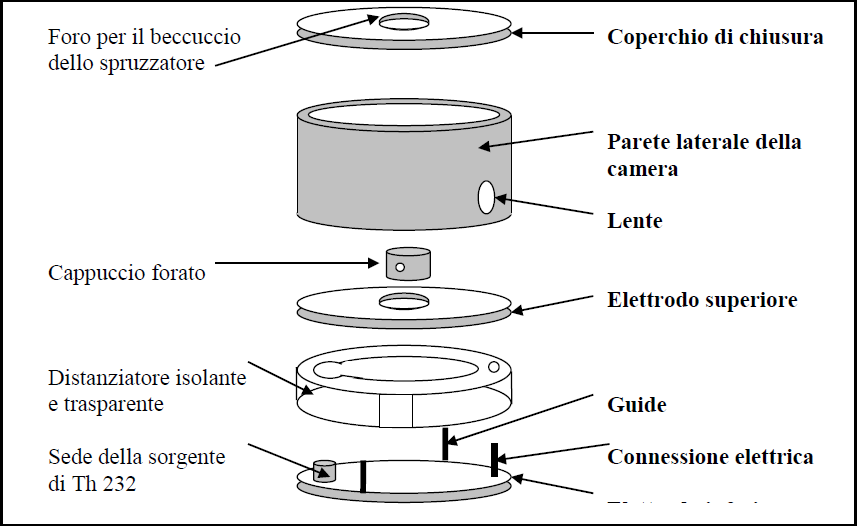
\includegraphics[width=0.6\textwidth]{Apparato2.png}
    \caption{Diagramma camera di Millikan con i suoi componenti principali.}
    \label{fig:camera_millikan}
\end{figure}

La camera è provvista di una parete laterale con una lente incorporata, che permette di visualizzare il comportamento delle gocce all'interno della camera. Accanto ad essa vi è un sistema di illuminazione basato su una lampada alogena, che facilita l’osservazione delle gocce di piccole dimensioni.

Prima di iniziare l’esperimento, è essenziale pulire e assemblare con attenzione l’apparato, rimuovendo eventuali residui derivanti dalle precedenti osservazioni. Successivamente, è necessario mettere in bolla lo strumento per garantire che le misurazioni non siano influenzate da inclinazioni. Dopo questa fase preliminare, l’ago in dotazione viene inserito nel foro dell'elettrodo superiore, e la lampada alogena viene accesa per illuminare la camera. A questo punto si mette a fuoco l’ago, insieme alla quadrettatura di fondo, che servirà come riferimento per calcolare la velocità delle gocce d'olio.

\begin{figure}[H]
    \centering
    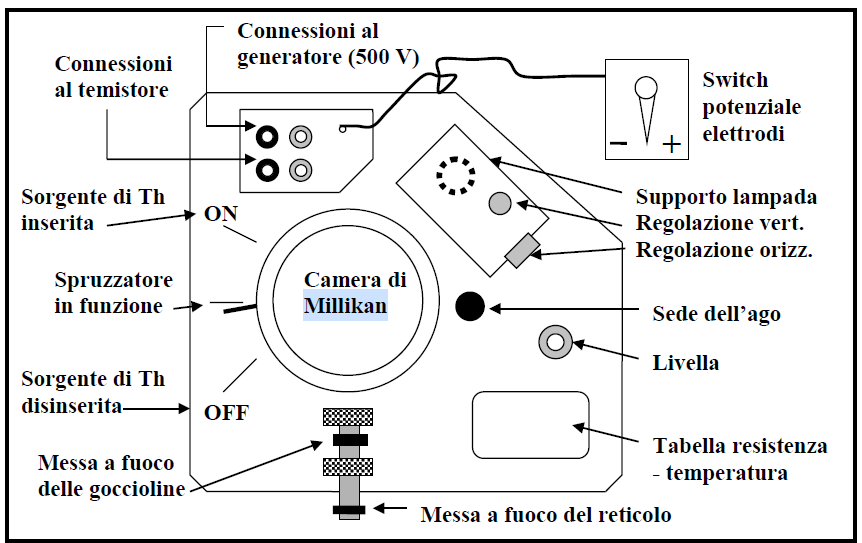
\includegraphics[width=0.7\textwidth]{Apparatopng.png}
    \caption{Vista dell'apparato completo, che include la camera di Millikan e le connessioni necessarie per l'osservazione e la regolazione.}
    \label{fig:apparato_completo}
\end{figure}

Una volta completata questa messa a punto, l’ago viene rimosso e si inserisce nuovamente il cappuccio nell’elettrodo superiore. Dopo aver completato questi passaggi, è possibile iniziare le misurazioni. Inizialmente, si osserva una goccia in caduta per effetto della forza di gravità. Accendendo il generatore di tensione, è possibile modificare il campo elettrico all'interno della camera e osservare come la goccia reagisce a tali variazioni.

Prima di ciascuna misurazione, viene registrata la temperatura, che influisce su alcuni parametri utilizzati nelle formule (ad esempio, il coefficiente di viscosità \(\eta\) dell'aria). La temperatura all'interno della camera di Millikan è stimabile tramite apposite tabelle di conversione, a partire dalla misurazione della resistenza elettrica di un termistore integrato nell’apparato, utilizzando un multimetro in modalità ohmetro.


\section{Presa dati}
È stato osservato il movimento di 10 gocce di olio. Prima di ogni misurazione è stata misurata la temperatura all'interno della camera ottenendo valori di temperatura compresi tra 23°C e 25°C.

Dopo aver spruzzato su un tovagliolo di carta per verificare la corretta fuoriuscita delle gocce, si inserisce il beccuccio nel foro del coperchio e osservando all’interno della camera si notano centinaia di gocce muoversi davanti ad un reticolo quadrettato posto sullo sfondo.

Dopo aver individuato una goccia che risponde adeguatamente al campo elettrico generato (può capitare che la goccia abbia carica neutra o che sia troppo pesante affinché il campo elettrico domini la forza di gravità), la si eleva di quota posizionandola in corrispondenza del lato superiore del primo quadretto e la si lascia in caduta. Si dimostra che la goccia, per effetto dell’attrito viscoso che stabilisce l’equilibrio delle forze, raggiunge una velocità limite in un tempo \( t = 10^{-5} \, \text{s} \), impercettibile all’occhio umano, muovendosi da quel momento di moto rettilineo uniforme. Attraverso un cronometro si misura il tempo impiegato dalla goccia a compiere ogni quadretto della dimensione \( \Delta z = 0.5 \, \text{mm} \), e sfruttando la relazione \( v = \frac{\Delta z}{t} \), si trova la velocità con cui la goccia percorre un quadretto. Facendo la media delle velocità nei cinque quadretti si ricava una miglior stima della velocità di caduta delle gocce.

Appena concluso il percorso di caduta della goccia sotto effetto della forza gravitazionale, prima che la goccia si depositi sul fondo della camera, viene causata la risalita della goccia attivando il generatore di tensione e impostando la corretta polarità degli elettrodi. Si eseguono le stesse misurazioni di distanza percorsa e relativo tempo di percorrenza per stimare la velocità in risalita della goccia sotto effetto di un campo elettrico verticale (bilanciato insieme alla forza di Archimede dalla forza peso e dalla forza di attrito viscoso, sempre in una condizione di moto rettilineo uniforme). Infine, si inverte il verso del campo elettrico operando lo switch del potenziale dei due elettrodi e procedendo a prendere le medesime misure del moto della goccia sotto effetto del campo elettrico anche in discesa.

La misurazione della velocità del moto delle gocce d’olio in caduta per effetto della gravità e in movimento per l’effetto del campo elettrico è legata rispettivamente all’obiettivo di ottenere una stima del raggio delle gocce e successivamente ricavare la loro carica elettrica per proseguire con la ricerca della stima finale della carica elementare.



\section{Misurazioni, Calcoli e Analisi Dati}

La prima misura eseguita nell'ambito dell'esperimento di Millikan riguarda lo spessore del distanziatore tra i due elettrodi, con l'obiettivo di calcolare il campo elettrico a partire dalla differenza di potenziale impostata tramite il generatore. Nel nostro esperimento, la misura dello spessore è stata effettuata utilizzando un calibro con sensibilità di \SI{0.1}{mm}, utilizzata come incertezza sulle misurazioni.

Le misurazioni dello spessore sono state effettuate in cinque punti diversi del distanziatore, ottenendo i valori riportati nella Tabella~\ref{tab:distanza_armature}.

\begin{table}[H]
    \centering
    \caption{Misure dello spessore del distanziatore tra gli elettrodi.}
    \label{tab:distanza_armature}
    \begin{tabular}{ccc S[table-format=1.2]}
    \toprule
    \textbf{Misura} & \textbf{$d$ [mm]} & $\sigma_d$ [mm] \\
    \midrule
    1 & 7.56 & 0.10 \\
    2 & 7.56 & 0.10 \\
    3 & 7.56 & 0.10 \\
    4 & 7.57 & 0.10 \\
    5 & 7.55 & 0.10 \\
    \bottomrule
    \end{tabular}
\end{table}


La media dei valori misurati fornisce la stima migliore dello spessore del distanziatore, mentre l'incertezza finale è stata calcolata come deviazione standard della media. Otteniamo così:
\begin{equation}
d = (0.00756 \pm 0.00005) \, \mathrm{m}
\label{eq:spessore_lamina}
\end{equation}

Conoscendo lo spessore \( d \), impostando una differenza di potenziale \( V \) (durante lo svolgimento abbiamo utilizzato tensioni comprese tra \SI{225}{V} e \SI{430}{V}, considerando un'incertezza sulla tensione pari a \SI{1}{V}, ossia l'unità dell'ultima cifra leggibile sul display del generatore di tensione), è possibile calcolare il modulo del campo elettrico \( E \) tra i due elettrodi utilizzando la relazione:
\begin{equation}
E= \frac{V}{d}
\label{eq:campo_elettrico}
\end{equation}

L'incertezza sul campo elettrico \( \sigma_E \) si ottiene tramite la propagazione delle incertezze di \( V \) e \( d \) nella formula (\ref{eq:campo_elettrico}):
\begin{equation}
\sigma_E= \sqrt{\left( \frac{\sigma_V}{d} \right)^2+ \left( \frac{V}{d^2} \sigma_d \right)^2}
\label{eq:incertezza_E}
\end{equation}

La velocità del moto rettilineo uniforme della goccia d’olio è stata calcolata a partire dalla distanza percorsa \( \Delta z = \SI{0.0005}{m} \), con un'incertezza \( \sigma_{\Delta z} = \SI{0.0001}{m} \) (pari al lato dei quadretti del reticolo di minore dimensione usato come riferimento per la misura delle distanze), e dal tempo \( \Delta t \) impiegato dalla goccia a percorrere tale distanza, misurato con un cronometro manuale. Su ogni intervallo di tempo misurato si è stimata, sulla base dei tempi di reazione umani, un'incertezza sullo start e sullo stop di \( \SI{0.2}{s} \), da cui si ottiene l'incertezza totale su \( \Delta t \):
\begin{equation}
\sigma_{\Delta t}= \sqrt{(\SI{0.2}{s})^2+ (\SI{0.2}{s})^2} \approx \SI{0.28}{s}
\label{eq:incertezza_tempo}
\end{equation}

La velocità della goccia è dunque:
\begin{equation}
v= \frac{\Delta z}{\Delta t}
\label{eq:velocita_goccia}
\end{equation}
con incertezza:
\begin{equation}
\sigma_v= \sqrt{\left( \frac{\sigma_{\Delta z}}{\Delta t} \right)^2+ \left( \frac{\Delta z}{\Delta t^2} \sigma_{\Delta t} \right)^2}
\label{eq:incertezza_velocita}
\end{equation}

Per ogni goccia considerata, sono state effettuate 5 misurazioni della velocità in caduta libera, da cui sono state calcolate 5 stime del raggio della goccia utilizzando la relazione derivata imponendo l'equilibrio tra le forze in gioco (forza peso, spinta di Archimede e forza di attrito viscoso):
\begin{equation}
r= \sqrt{\left( \frac{b}{2p} \right)^2+ \frac{9 \eta v^2}{g(\rho_{\text{olio}} - \rho_{\text{aria}})}} - \frac{b}{2p}
\label{eq:raggio_goccia}
\end{equation}
dove:
\begin{itemize}
\item \( \eta \) è il coefficiente di viscosità dell'aria, calcolato a partire dalla temperatura \( T \) all'interno della camera di Millikan tramite la relazione:
\begin{equation}
\eta(T) = [1.800 + 4.765 \times 10^{-3} (T - 15^\circ \text{C})] \times 10^{-5} \, \text{N}\cdot\text{s}\cdot\text{m}^{-2}
\label{eq:viscosita}
\end{equation}
\item \( b \) è un parametro empirico di correzione del coefficiente di viscosità noto essere \( 8.2 \times 10^{-3} \, \text{Pa} \cdot \text{m} \), con incertezza supposta trascurabile.
\item \( p = \SI{101325}{Pa} \) è la pressione atmosferica.
\item \( g = \SI{9.806}{m/s^2} \) è l'accelerazione di gravità a Milano, la cui incertezza è trascurabile.
\item \( \rho_{\text{olio}} = \SI{860}{kg/m^3} \) e \( \rho_{\text{aria}} = \SI{1.293}{kg/m^3} \) sono le densità dell'olio e dell'aria rispettivamente.
\end{itemize}

Per le misurazioni della temperatura all’interno della camera di Millikan ogni volta ottenute misurando la resistenza elettrica del termistore dell’apparato tramite un multimetro e consultando le apposite tabelle di conversione della resistenza in corrispondenti valori di temperatura, si è stimata un’incertezza di \( \sigma_T = \SI{0.5}{^\circ C} \), considerando le imprecisioni dovute all’oscillazione del valore della resistenza indicato sul multimetro e alla non sempre totale corrispondenza tra valore letto sullo strumento e valore della resistenza consultabile sulla tabella di conversione. 

L'incertezza sul coefficiente di viscosità \( \sigma_{\eta} \) è stata calcolata propagando l'incertezza sulla temperatura nella formula (\ref{eq:viscosita}):
\begin{equation}
\sigma_{\eta} = 4.765 \times 10^{-8} \, \sigma_T
\label{eq:incertezza_viscosita}
\end{equation}

L'incertezza sul raggio \( \sigma_r \) è stata ottenuta tramite la propagazione delle incertezze di \( v \) e \( \eta \) nella formula (\ref{eq:raggio_goccia}):
\begin{equation}
\sigma_r = \sqrt{\left( \frac{\partial r}{\partial v} \sigma_v \right)^2 + \left( \frac{\partial r}{\partial \eta} \sigma_{\eta} \right)^2}
\label{eq:incertezza_raggio}
\end{equation}
dove le derivate parziali sono calcolate rispetto alla formula (\ref{eq:raggio_goccia}).

Ottenute le 5 misurazioni del raggio per ogni goccia, si è eseguita una media pesata per determinare la stima migliore del raggio di ciascuna goccia, con relativa incertezza.

Successivamente, si è stimata la carica di ogni goccia utilizzando le misure del raggio precedentemente ottenute. Sono state effettuate 5 misurazioni della velocità della goccia durante la salita all'interno della camera sotto l'effetto del campo elettrico (generato applicando una differenza di potenziale \( V \)), e altre 5 misurazioni durante la discesa invertendo il segno della tensione. In totale, per ciascuna delle 10 gocce considerate, sono state ottenute 10 misurazioni della carica.

La carica \( Q \) della goccia è stata calcolata, nel caso in cui la goccia sale, utilizzando la formula:
\begin{equation}
Q= -\frac{4}{3} \pi r^3 (\rho_{\text{olio}} - \rho_{\text{aria}}) \frac{g}{E} \left(1 + \frac{|v_E|}{v_0}\right)
\label{eq:carica_goccia_sale}
\end{equation}
dove:
\begin{itemize}
\item \( E = \frac{V}{d} \) è il campo elettrico applicato.
\item \( r \) è il raggio della goccia calcolato.
\item \( v_E \) è la velocità della goccia in presenza del campo elettrico.
\item \( v_0 \) è il valore della velocità precedentemente misurato della goccia in caduta per effetto della sola gravità (è stata in particolare usata la media delle 5 misurazioni di $v_0$ ottenute). 
\end{itemize}

L'incertezza sulla carica \( \sigma_Q \) è stata calcolata propagando le incertezze sulle quantità misurate:
\begin{equation}
\sigma_Q = \sqrt{\left( \frac{\partial Q}{\partial r} \sigma_r \right)^2 + \left( \frac{\partial Q}{\partial E} \sigma_E \right)^2 + \left( \frac{\partial Q}{\partial v_E} \sigma_{v_E} \right)^2 + \left( \frac{\partial Q}{\partial v_0} \sigma_{v_0} \right)^2}
\label{eq:incertezza_carica}
\end{equation}

Nel caso in cui la goccia scende sotto l'effetto del campo elettrico, la formula diventa:
\begin{equation}
Q= -\frac{4}{3} \pi r^3 (\rho_{\text{olio}} - \rho_{\text{aria}}) \frac{g}{E} \left(1 - \frac{|v_E|}{v_0}\right)
\label{eq:carica_goccia_scende}
\end{equation}
Le incertezze sono calcolate in modo analogo.

In totale, per le 10 gocce analizzate, sono stati ottenuti 100 valori di carica elettrica.

Di seguito, riportiamo un esempio di misure e calcoli per lo studio di una goccia.

\subsection{Esempio di calcolo per una goccia}

\subsubsection{Misure in caduta libera (\( \Delta V = 0 \))}

Le misure del tempo di caduta \( t \) e le velocità calcolate sono riportate nella Tabella~\ref{tab:caduta_libera}. La temperatura durante le misurazioni era di \( T = 23 \, ^\circ\text{C} \) con un'incertezza di \( \sigma_T = 0.5 \, ^\circ\text{C} \). La viscosità dell'aria è stata considerata costante a \( \eta = 1.84 \times 10^{-5} \, \text{Ns/m}^2 \) con un'incertezza di \( \sigma_\eta = 2.38 \times 10^{-8} \, \text{Ns/m}^2 \).

\begin{table}[H]
    \centering
    \caption{Misure con $\Delta V = 0$}
    \label{tab:caduta_libera}
    \begin{tabular}{cccccc}
    \toprule
    \textbf{t [s]} & \textbf{$\sigma_t$} & \textbf{$v_0$ [m/s]} & \textbf{$\sigma_{v_0}$}\footnote{Le incertezze sulle velocità \( \sigma_{v_0} \) sono calcolate utilizzando la formula (\ref{eq:incertezza_velocita}).} & \textbf{r [m]} & \textbf{$\sigma_r$} \\
    \midrule
    35,2 & 0,3 & 1,42E-05 & 2,8E-06 & 3,4E-07 & 4E-08 \\
    82,4 & 0,3 & 1,06E-05 & 2,1E-06 & 2,9E-07 & 3E-08 \\
    128,0 & 0,3 & 1,10E-05 & 2,2E-06 & 2,9E-07 & 3E-08 \\
    174,1 & 0,3 & 1,08E-05 & 2,2E-06 & 2,9E-07 & 3E-08 \\
    221,8 & 0,3 & 1,05E-05 & 2,1E-06 & 2,8E-07 & 3E-08 \\
    \midrule
    \textbf{Medio} & & 1,11E-05 & 1,0E-06 & 2,87-07 & 1,6E-08 \\
    \bottomrule
    \end{tabular}
\end{table}

Il valor medio della velocità \( v_0 \), del raggio \( r \)  e le relative incertezze sono state calcolate come media pesata delle misure.


\subsubsection{Misure con campo elettrico (\( \Delta V = \SI{430}{V} \))}

Le misure del tempo \( t \) e delle velocità \( v \) calcolate per le gocce sotto l'effetto di un campo elettrico sono riportate nella Tabella~\ref{tab:campo_elettrico_goccia_sale}. Il campo elettrico \( E \) generato è pari a \( 5.6878 \times 10^4 \, \text{Vm}^{-1} \) con un'incertezza di \( \sigma_E = 2.07 \times 10^{-2} \, \text{Vm}^{-1} \).

\begin{table}[H]
    \centering
    \caption{Misure con $\Delta V = 430$}
    \label{tab:campo_elettrico_goccia_sale}
    \begin{tabular}{cccccc}
    \toprule
    \textbf{t [s]} & \textbf{$\sigma_t$} & \textbf{v [m/s]} & \textbf{$\sigma_v$} & \textbf{Q [C]} & \textbf{$\sigma_Q$} \\
    \midrule
    4,2 & 0,3 & 1,18E-4 & 2,5E-5 & 1,5E-19 & 6E-20 \\
    8,9 & 0,3 & 1,08E-4 & 2,3E-5 & 1,3E-19 & 4E-20 \\
    12,8 & 0,3 & 1,27E-4 & 2,7E-5 & 1,6E-19 & 5E-20 \\
    16,9 & 0,3 & 1,21E-4 & 2,6E-5 & 1,5E-19 & 5E-20 \\
    20,9 & 0,3 & 1,25E-4 & 2,7E-5 & 1,E-19 & 5E-20 \\
    \bottomrule
    \end{tabular}
\end{table}

\subsubsection{Misure con campo elettrico (\( \Delta V = \SI{-430}{V} \))}

Le misure del tempo \( t \) e delle velocità \( v \) calcolate per le gocce sotto l'effetto di un campo elettrico mentre la goccia sale sono riportate nella Tabella~\ref{tab:campo_elettrico_goccia_sale}.  Il campo elettrico generato è pari a quello della precedente misurazione, ma di segno opposto.

\begin{table}[H]
    \centering
    \caption{Misure con $\Delta V = -430$}
    \label{tab:campo_elettrico_goccia_sale}
    \begin{tabular}{cccccc}
    \toprule
    \textbf{t [s]} & \textbf{$\sigma_t$} & \textbf{v [m/s]} & \textbf{$\sigma_v$} & \textbf{Q [C]} & \textbf{$\sigma_Q$} \\
    \midrule
    5,0 & 0,3 & 9,98E-5 & 2,1E-5 & 1,50E-19 & 5E-20 \\
    10,3 & 0,3 & 9,51E-5 & 2,0E-5 & 1,36E-19 & 4E-20 \\
    15,9 & 0,3 & 8,87E-5 & 1,8E-5 & 1,3E-19 & 4E-20 \\
    21,5 & 0,3 & 8,94E-5 & 1,9E-5 & 1,29E-19 & 4E-20 \\
    28,5 & 0,3 & 7,13E-5 & 1,5E-5 & 1,06E-19 & 3E-20 \\
    \bottomrule
    \end{tabular}
\end{table}

Da notare come alcune di queste misure siano fuori scala rispetto alle altre, come la prima della Tabella~\ref{tab:caduta_libera}, e siano state perciò scartate. 


\subsection{Cariche otteute}
Iterato questo procedimento per 10 gocce diverse abbiamo ottenuto i dati raffigurati nell'istogramma \ref{fig:Istogramma}
\begin{figure}[H]
    \centering
    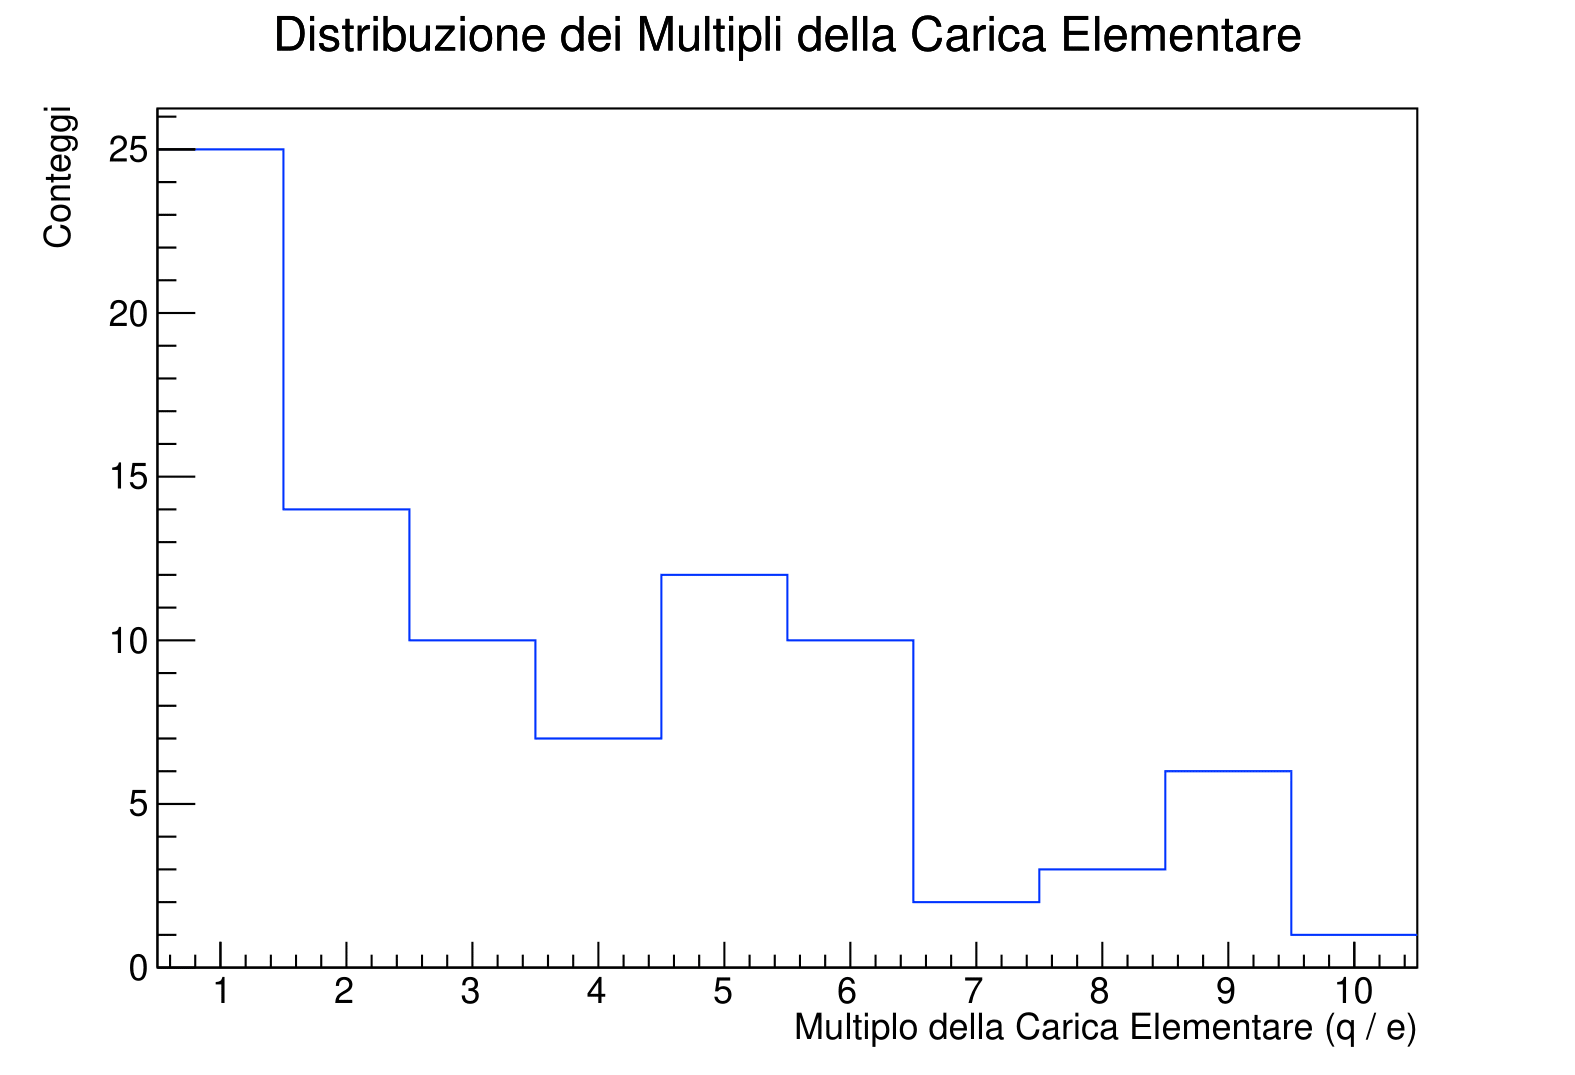
\includegraphics[width=0.7\textwidth]{Istogramma.png}
    \caption{Multiplo di cariche elementari delle gocce studiate}
    \label{fig:Istogramma}
\end{figure}
Attraverso questo istogramma è possibile constatare che più di un quarto delle gocce studiate presentava una carica pari a quella elementare, cioè non è stato necessario dividere per alcun valore quanto ottenuto.

\section{Stima finale della carica elementare}

Come è noto, il valore della carica elettrica delle gocce d’olio prese in considerazione, così come per ogni corpo elettricamente carico, deve necessariamente essere esprimibile come multiplo intero della carica elementare dell’elettrone.

Per la stima della carica dell’elettrone sono stati messi in relazione i valori delle cariche misurate delle gocce d’olio con valori di carica compresi in un range di \([1.400 \times 10^{-19} \, \text{C}, \, 1.800 \times 10^{-19} \, \text{C}]\), con l’obiettivo di individuare quale valore di carica elettrica all’interno del range è stimabile con la migliore approssimazione come rapporto tra le cariche misurate e un opportuno intero.

Dunque, si considera, al variare del valore di carica \( q \) appartenente al range indicato, la seguente quantità \( S(q) \), che rappresenta una funzione di \( q \in [1.400 \times 10^{-19} \, \text{C}, \, 1.800 \times 10^{-19} \, \text{C}] \):
\begin{equation}
S(q) = \sum_{i=1}^{N} \left( \frac{Q_i}{k_i(q)}- q \right)^2
\label{eq:somma_scarti}
\end{equation}
dove:
\begin{itemize}
\item \( Q_i \) indica l’i-esimo valore di carica misurato.
\item \( k_i \) rappresenta il numero intero più vicino al rapporto \( Q_i / q \), ottenuto calcolando la parte intera della quantità \( \left( Q_i / q + 0.5 \right) \).
\end{itemize}

Il valore di carica \( q \) che minimizza la quantità \( S(q) \) è il valore di carica che consente di esprimere le cariche \( Q_i \) come multiplo intero (tramite l’intero \( k_i \) stimato) di \( q \) con la migliore approssimazione; dunque, rappresenta il valore della carica elementare.

\begin{figure}[H]
    \centering
    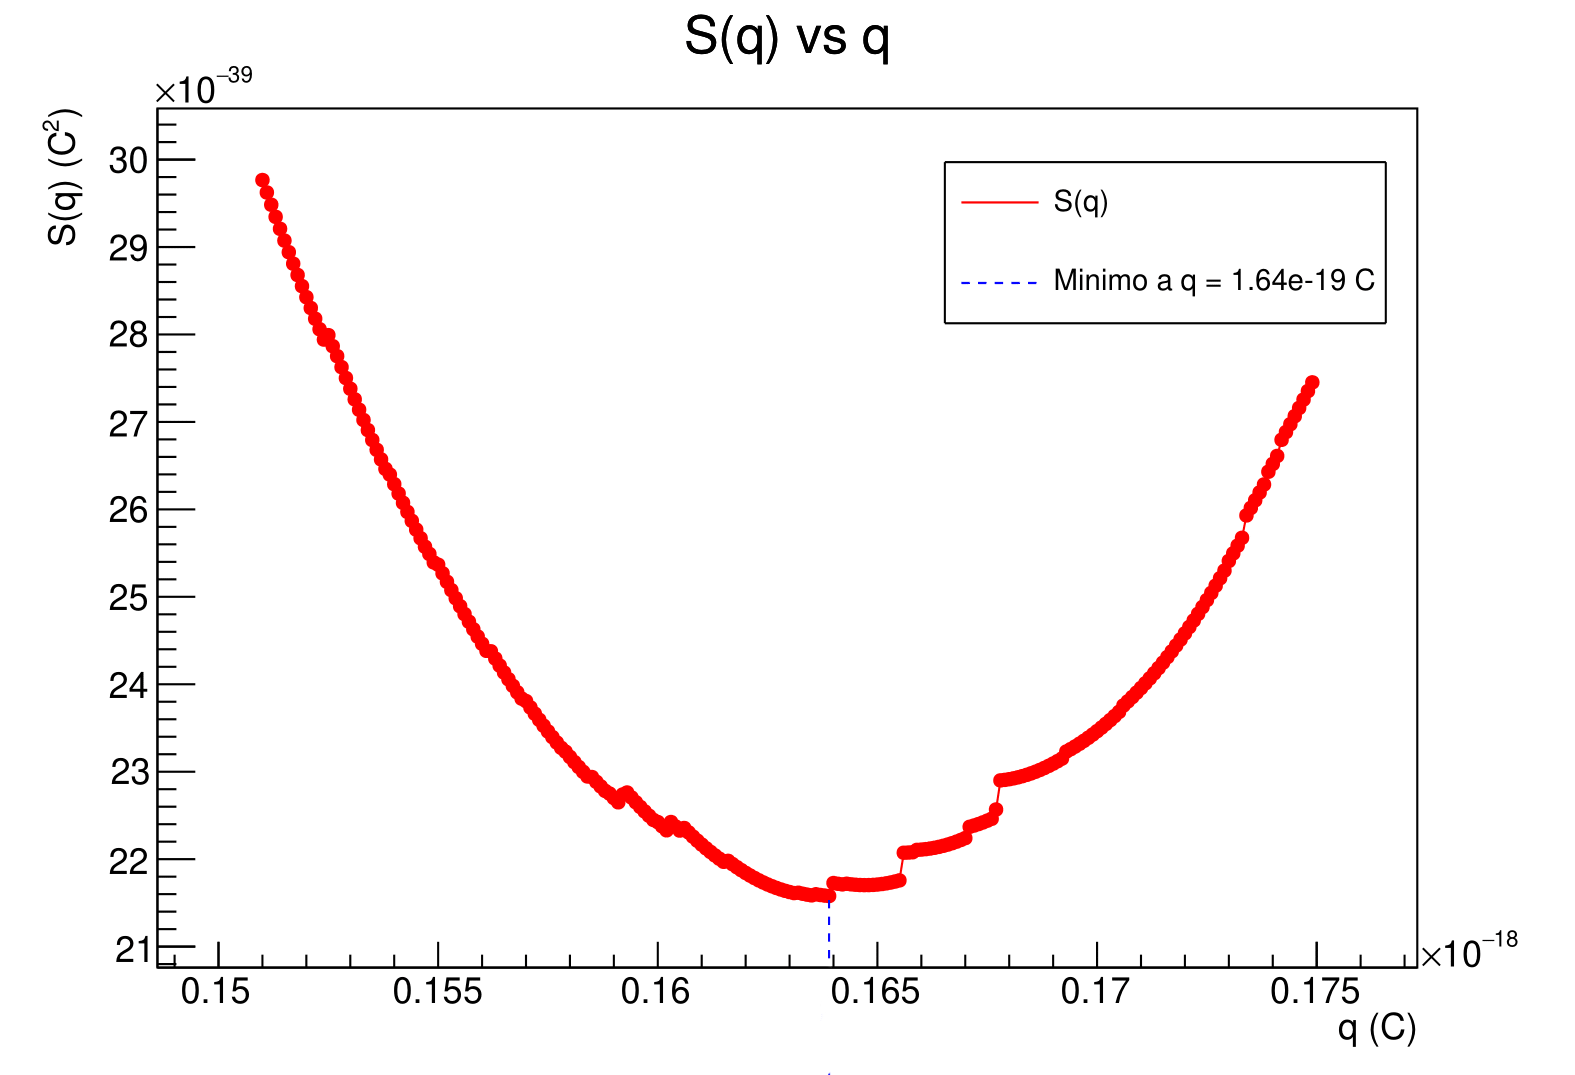
\includegraphics[width=0.7\textwidth]{GraficoSFunction.png}
    \caption{Grafico della funzione \( S(q) \) per la determinazione della carica elementare. Il punto di minimo rappresenta la stima di \( q_e \).}
    \label{fig:minimo_Sq}
\end{figure}

Il valore della carica elementare che corrisponde al punto di minimo della funzione \( S(q) \), è ottenibile valutando il valore di \( q \) che annulla la derivata prima della funzione:
\begin{equation}
\frac{dS(q)}{dq} = 2 \sum_{i=1}^{N} \left( \frac{Q_i}{k_i} - q \right) = 0 \quad \Rightarrow \quad q_e = \frac{1}{N}\sum_{i=1}^{N}{ \frac {Q_i} {k_i}}
\label{eq:minimizzazione_Sq}
\end{equation}

È dunque possibile stimare la sua incertezza come la deviazione standard della media dei rapporti \(Q_i/k_i\):
\begin{equation}
\sigma_{q_e} = \sqrt{\frac{S(q_e)}{N(N-1)}}
\label{eq:incertezza_qe}
\end{equation}

È stata dunque ottenuta la seguente misura della carica dell’elettrone:
\begin{equation}
q_e = - (1,641 \pm 0,016) \times 10^{-19} \, \text{C}
\label{eq:carica_elementare}
\end{equation}

Individuando un intervallo di confidenza di:
\begin{equation}
[-1,625 \times 10^{-19} \, \text{C}, \, -1,657 \times 10^{-19} \, \text{C}]
\end{equation}

Si è dunque successivamente calcolata la compatibilità della misura ottenuta della carica elementare con il valore universalmente noto di, 
\( -1,6022 \times 10^{-19} \, \text{C} \), ottenendo una compatibilità del 
\( 1,83 \, \% \). 
Un tale livello di compatibilità rappresenta comunque un risultato soddisfacente dal momento che può essere ulteriormente migliorato riducendo gli errori casuali, legati principalmente ai limiti dell’osservazione umana e riducibili adottando procedimenti di misura più avanzati. La difficoltà nel selezionare una singola goccia e seguirne con precisione il movimento per diversi minuti, mantenendo un livello di attenzione elevato, e l’immediata comunicazione che è necessario mantenere tra l’osservatore e il collaboratore che gestisce il cronometro, può rendere questo procedimento di misurazione soggetto ad un errore considerevole. Potrebbe risultare possibile ridurre queste fonti di errore ad esempio osservando il moto delle gocce registrando filmati ad alta risoluzione, eventualmente anche a rallentatore, dei moti delle gocce che avvengono nella camera, con maggiori possibilità di raccogliere le misure temporali con maggiore accuratezza e di individuare con minore incertezza la posizione delle gocce d’olio e quindi i loro spostamenti; in aggiunta, si ridurrebbe notevolmente la componente di errore dovuta alla fatica degli osservatori. Inoltre, aumentando il numero di misurazioni, si potrebbe migliorare ulteriormente la compatibilità dei risultati con il valore teorico della carica elementare.


\end{document}
